
\lecture{t tables}{t-tables}
\section{t Tables}

\title{t Tables}
\subtitle{More numbers than you can shake a stick at}

%\author{Kelly Black}
%\institute{Clarkson University}
\date{11 November 2013}

\begin{frame}
  \titlepage
\end{frame}

\begin{frame}
  \frametitle{Outline}
  \tableofcontents[hideothersubsections,sectionstyle=show/hide]
\end{frame}


\subsection{t Tables}


\subsection{Approximating Probabilities with Tables}

\begin{frame}{Calculating the Probability For the Standard Normal}

  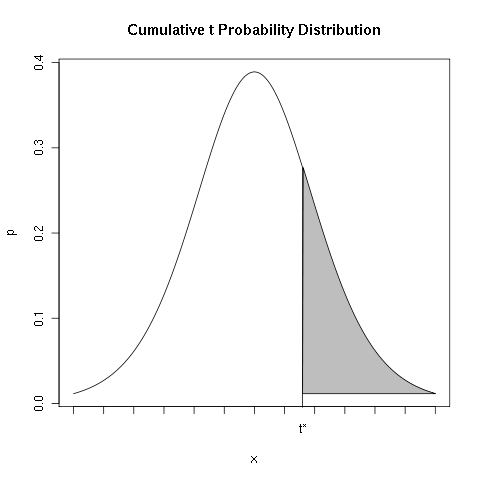
\includegraphics[width=6cm]{img/tcummulativeDist}
  
\end{frame}

\begin{frame}
  \frametitle{The Critical $t$-Table}
  \vspace*{-5em}
  \hfill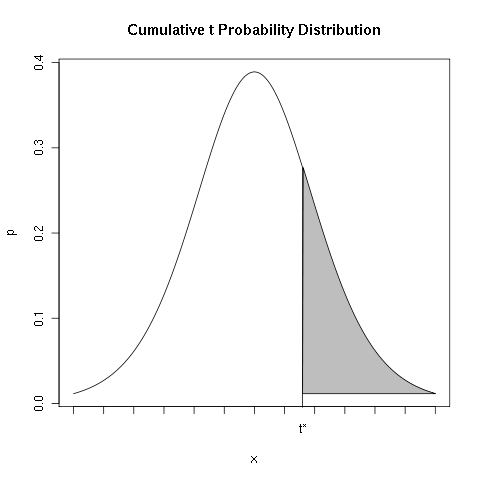
\includegraphics[width=2cm]{img/tcummulativeDist}~~~~~~~~~~~~~~

  {
\fontencoding{T1}
\fontfamily{pcr}
\fontseries{m}
\fontshape{n}
\fontsize{5pt}{5pt}
\selectfont
\begin{tabular}{l|llllllllllll} 
df  & p= 0.2500  &  0.2000  &  0.1500  &  0.1000  &  0.0500  &  0.0250  &  0.0200  &  0.0100  &  0.0050    \\\hline 
  1 & 1.0000 & 1.3764 & 1.9626 & 3.0777 & 6.3138 & 12.7062 & 15.8945 & 31.8205 & 63.6567  \\[5pt] \arrayrulecolor{light-gray}\hline\arrayrulecolor{black}  
  2 & 0.8165 & 1.0607 & 1.3862 & 1.8856 & 2.9200 & 4.3027 & 4.8487 & 6.9646 & 9.9248  \\[5pt] \arrayrulecolor{light-gray}\hline\arrayrulecolor{black}  
  3 & 0.7649 & 0.9785 & 1.2498 & 1.6377 & 2.3534 & 3.1824 & 3.4819 & 4.5407 & 5.8409  \\[5pt] \arrayrulecolor{light-gray}\hline\arrayrulecolor{black}  
  4 & 0.7407 & 0.9410 & 1.1896 & 1.5332 & 2.1318 & 2.7764 & 2.9985 & 3.7469 & 4.6041  \\[12pt] \arrayrulecolor{light-gray}\hline\arrayrulecolor{black}  
  5 & 0.7267 & 0.9195 & 1.1558 & 1.4759 & 2.0150 & 2.5706 & 2.7565 & 3.3649 & 4.0321  \\[5pt] \arrayrulecolor{light-gray}\hline\arrayrulecolor{black}  
  6 & 0.7176 & 0.9057 & 1.1342 & 1.4398 & 1.9432 & 2.4469 & 2.6122 & 3.1427 & 3.7074  \\[5pt] \arrayrulecolor{light-gray}\hline\arrayrulecolor{black}  
  7 & 0.7111 & 0.8960 & 1.1192 & 1.4149 & 1.8946 & 2.3646 & 2.5168 & 2.9980 & 3.4995  \\[5pt] \arrayrulecolor{light-gray}\hline\arrayrulecolor{black}  
  8 & 0.7064 & 0.8889 & 1.1081 & 1.3968 & 1.8595 & 2.3060 & 2.4490 & 2.8965 & 3.3554  \\[5pt] \arrayrulecolor{light-gray}\hline\arrayrulecolor{black}  
  9 & 0.7027 & 0.8834 & 1.0997 & 1.3830 & 1.8331 & 2.2622 & 2.3984 & 2.8214 & 3.2498  \\[12pt] \arrayrulecolor{light-gray}\hline\arrayrulecolor{black}  
 10 & 0.6998 & 0.8791 & 1.0931 & 1.3722 & 1.8125 & 2.2281 & 2.3593 & 2.7638 & 3.1693  \\[5pt] \arrayrulecolor{light-gray}\hline\arrayrulecolor{black}  
 11 & 0.6974 & 0.8755 & 1.0877 & 1.3634 & 1.7959 & 2.2010 & 2.3281 & 2.7181 & 3.1058  \\[5pt] \arrayrulecolor{light-gray}\hline\arrayrulecolor{black}  
 12 & 0.6955 & 0.8726 & 1.0832 & 1.3562 & 1.7823 & 2.1788 & 2.3027 & 2.6810 & 3.0545  \\[5pt] \arrayrulecolor{light-gray}\hline\arrayrulecolor{black}  
 13 & 0.6938 & 0.8702 & 1.0795 & 1.3502 & 1.7709 & 2.1604 & 2.2816 & 2.6503 & 3.0123  \\[5pt] \arrayrulecolor{light-gray}\hline\arrayrulecolor{black}  
 14 & 0.6924 & 0.8681 & 1.0763 & 1.3450 & 1.7613 & 2.1448 & 2.2638 & 2.6245 & 2.9768  \\[12pt] \arrayrulecolor{light-gray}\hline\arrayrulecolor{black}  
 15 & 0.6912 & 0.8662 & 1.0735 & 1.3406 & 1.7531 & 2.1314 & 2.2485 & 2.6025 & 2.9467  \\[5pt] \arrayrulecolor{light-gray}\hline\arrayrulecolor{black}  
 16 & 0.6901 & 0.8647 & 1.0711 & 1.3368 & 1.7459 & 2.1199 & 2.2354 & 2.5835 & 2.9208  \\[5pt] \arrayrulecolor{light-gray}\hline\arrayrulecolor{black}  
 17 & 0.6892 & 0.8633 & 1.0690 & 1.3334 & 1.7396 & 2.1098 & 2.2238 & 2.5669 & 2.8982  \\[5pt] \arrayrulecolor{light-gray}\hline\arrayrulecolor{black}  
 18 & 0.6884 & 0.8620 & 1.0672 & 1.3304 & 1.7341 & 2.1009 & 2.2137 & 2.5524 & 2.8784  \\[5pt] \arrayrulecolor{light-gray}\hline\arrayrulecolor{black}  
\end{tabular}
}
\end{frame}


\subsection{Examples}

\begin{frame}{\small Find the value of $t$ for a $t$ distribution with
    12 degrees of freedom where the area to the left is 0.05.}
  
{\small First find the row corresponding to 12 degrees of freedom.}

  {
\fontencoding{T1}
\fontfamily{pcr}
\fontseries{m}
\fontshape{n}
\fontsize{5pt}{5pt}
\selectfont
\begin{tabular}{l|llllllllllll} 
df  & p= 0.2500  &  0.2000  &  0.1500  &  0.1000  &  0.0500  &  0.0250  &  0.0200  &  0.0100  &  0.0050     \\\hline 
  1 & 1.0000 & 1.3764 & 1.9626 & 3.0777 & 6.3138 & 12.7062 & 15.8945 & 31.8205 & 63.6567  \\[5pt] \arrayrulecolor{light-gray}\hline\arrayrulecolor{black}  
  2 & 0.8165 & 1.0607 & 1.3862 & 1.8856 & 2.9200 & 4.3027 & 4.8487 & 6.9646 & 9.9248  \\[5pt] \arrayrulecolor{light-gray}\hline\arrayrulecolor{black}  
  3 & 0.7649 & 0.9785 & 1.2498 & 1.6377 & 2.3534 & 3.1824 & 3.4819 & 4.5407 & 5.8409  \\[5pt] \arrayrulecolor{light-gray}\hline\arrayrulecolor{black}  
  4 & 0.7407 & 0.9410 & 1.1896 & 1.5332 & 2.1318 & 2.7764 & 2.9985 & 3.7469 & 4.6041  \\[12pt] \arrayrulecolor{light-gray}\hline\arrayrulecolor{black}  
  5 & 0.7267 & 0.9195 & 1.1558 & 1.4759 & 2.0150 & 2.5706 & 2.7565 & 3.3649 & 4.0321  \\[5pt] \arrayrulecolor{light-gray}\hline\arrayrulecolor{black}  
  6 & 0.7176 & 0.9057 & 1.1342 & 1.4398 & 1.9432 & 2.4469 & 2.6122 & 3.1427 & 3.7074  \\[5pt] \arrayrulecolor{light-gray}\hline\arrayrulecolor{black}  
  7 & 0.7111 & 0.8960 & 1.1192 & 1.4149 & 1.8946 & 2.3646 & 2.5168 & 2.9980 & 3.4995  \\[5pt] \arrayrulecolor{light-gray}\hline\arrayrulecolor{black}  
  8 & 0.7064 & 0.8889 & 1.1081 & 1.3968 & 1.8595 & 2.3060 & 2.4490 & 2.8965 & 3.3554  \\[5pt] \arrayrulecolor{light-gray}\hline\arrayrulecolor{black}  
  9 & 0.7027 & 0.8834 & 1.0997 & 1.3830 & 1.8331 & 2.2622 & 2.3984 & 2.8214 & 3.2498  \\[12pt] \arrayrulecolor{light-gray}\hline\arrayrulecolor{black}  
 10 & 0.6998 & 0.8791 & 1.0931 & 1.3722 & 1.8125 & 2.2281 & 2.3593 & 2.7638 & 3.1693  \\[5pt] \arrayrulecolor{light-gray}\hline\arrayrulecolor{black}  
 11 & 0.6974 & 0.8755 & 1.0877 & 1.3634 & 1.7959 & 2.2010 & 2.3281 & 2.7181 & 3.1058  \\[5pt] \arrayrulecolor{light-gray}\hline\arrayrulecolor{black}  
\rowcolor{light-red} 12 & 0.6955 & 0.8726 & 1.0832 & 1.3562 & 1.7823 & 2.1788 & 2.3027 & 2.6810 & 3.0545  \\[5pt] \arrayrulecolor{light-gray}\hline\arrayrulecolor{black}  
 13 & 0.6938 & 0.8702 & 1.0795 & 1.3502 & 1.7709 & 2.1604 & 2.2816 & 2.6503 & 3.0123  \\[5pt] \arrayrulecolor{light-gray}\hline\arrayrulecolor{black}  
 14 & 0.6924 & 0.8681 & 1.0763 & 1.3450 & 1.7613 & 2.1448 & 2.2638 & 2.6245 & 2.9768  \\[12pt] \arrayrulecolor{light-gray}\hline\arrayrulecolor{black}  
 15 & 0.6912 & 0.8662 & 1.0735 & 1.3406 & 1.7531 & 2.1314 & 2.2485 & 2.6025 & 2.9467  \\[5pt] \arrayrulecolor{light-gray}\hline\arrayrulecolor{black}  
 16 & 0.6901 & 0.8647 & 1.0711 & 1.3368 & 1.7459 & 2.1199 & 2.2354 & 2.5835 & 2.9208  \\[5pt] \arrayrulecolor{light-gray}\hline\arrayrulecolor{black}  
 17 & 0.6892 & 0.8633 & 1.0690 & 1.3334 & 1.7396 & 2.1098 & 2.2238 & 2.5669 & 2.8982  \\[5pt] \arrayrulecolor{light-gray}\hline\arrayrulecolor{black}  
 18 & 0.6884 & 0.8620 & 1.0672 & 1.3304 & 1.7341 & 2.1009 & 2.2137 & 2.5524 & 2.8784  \\[5pt] \arrayrulecolor{light-gray}\hline\arrayrulecolor{black}  
\end{tabular}
}


\end{frame}

\begin{frame}{\small Find the value of $t$ for a $t$ distribution with
    12 degrees of freedom where the area to the left is 0.05.}
  
{\small First find the row corresponding to 12 degrees of freedom. Then
find the column associated with 0.05.}

  {
\fontencoding{T1}
\fontfamily{pcr}
\fontseries{m}
\fontshape{n}
\fontsize{5pt}{5pt}
\selectfont
\begin{tabular}{l|llll>{\columncolor{light-blue}}llllllll} 
df  & p= 0.2500  &  0.2000  &  0.1500  &  0.1000  &  0.0500  &  0.0250  &  0.0200  &  0.0100  &  0.0050   \\\hline 
  1 & 1.0000 & 1.3764 & 1.9626 & 3.0777 & 6.3138 & 12.7062 & 15.8945 & 31.8205 & 63.6567  \\[5pt] \arrayrulecolor{light-gray}\hline\arrayrulecolor{black}  
  2 & 0.8165 & 1.0607 & 1.3862 & 1.8856 & 2.9200 & 4.3027 & 4.8487 & 6.9646 & 9.9248  \\[5pt] \arrayrulecolor{light-gray}\hline\arrayrulecolor{black}  
  3 & 0.7649 & 0.9785 & 1.2498 & 1.6377 & 2.3534 & 3.1824 & 3.4819 & 4.5407 & 5.8409  \\[5pt] \arrayrulecolor{light-gray}\hline\arrayrulecolor{black}  
  4 & 0.7407 & 0.9410 & 1.1896 & 1.5332 & 2.1318 & 2.7764 & 2.9985 & 3.7469 & 4.6041  \\[12pt] \arrayrulecolor{light-gray}\hline\arrayrulecolor{black}  
  5 & 0.7267 & 0.9195 & 1.1558 & 1.4759 & 2.0150 & 2.5706 & 2.7565 & 3.3649 & 4.0321  \\[5pt] \arrayrulecolor{light-gray}\hline\arrayrulecolor{black}  
  6 & 0.7176 & 0.9057 & 1.1342 & 1.4398 & 1.9432 & 2.4469 & 2.6122 & 3.1427 & 3.7074  \\[5pt] \arrayrulecolor{light-gray}\hline\arrayrulecolor{black}  
  7 & 0.7111 & 0.8960 & 1.1192 & 1.4149 & 1.8946 & 2.3646 & 2.5168 & 2.9980 & 3.4995  \\[5pt] \arrayrulecolor{light-gray}\hline\arrayrulecolor{black}  
  8 & 0.7064 & 0.8889 & 1.1081 & 1.3968 & 1.8595 & 2.3060 & 2.4490 & 2.8965 & 3.3554  \\[5pt] \arrayrulecolor{light-gray}\hline\arrayrulecolor{black}  
  9 & 0.7027 & 0.8834 & 1.0997 & 1.3830 & 1.8331 & 2.2622 & 2.3984 & 2.8214 & 3.2498  \\[12pt] \arrayrulecolor{light-gray}\hline\arrayrulecolor{black}  
 10 & 0.6998 & 0.8791 & 1.0931 & 1.3722 & 1.8125 & 2.2281 & 2.3593 & 2.7638 & 3.1693  \\[5pt] \arrayrulecolor{light-gray}\hline\arrayrulecolor{black}  
 11 & 0.6974 & 0.8755 & 1.0877 & 1.3634 & 1.7959 & 2.2010 & 2.3281 & 2.7181 & 3.1058  \\[5pt] \arrayrulecolor{light-gray}\hline\arrayrulecolor{black}  
\rowcolor{light-red} 12 & 0.6955 & 0.8726 & 1.0832 & 1.3562 & 1.7823 & 2.1788 & 2.3027 & 2.6810 & 3.0545  \\[5pt] \arrayrulecolor{light-gray}\hline\arrayrulecolor{black}  
 13 & 0.6938 & 0.8702 & 1.0795 & 1.3502 & 1.7709 & 2.1604 & 2.2816 & 2.6503 & 3.0123  \\[5pt] \arrayrulecolor{light-gray}\hline\arrayrulecolor{black}  
 14 & 0.6924 & 0.8681 & 1.0763 & 1.3450 & 1.7613 & 2.1448 & 2.2638 & 2.6245 & 2.9768  \\[12pt] \arrayrulecolor{light-gray}\hline\arrayrulecolor{black}  
 15 & 0.6912 & 0.8662 & 1.0735 & 1.3406 & 1.7531 & 2.1314 & 2.2485 & 2.6025 & 2.9467  \\[5pt] \arrayrulecolor{light-gray}\hline\arrayrulecolor{black}  
 16 & 0.6901 & 0.8647 & 1.0711 & 1.3368 & 1.7459 & 2.1199 & 2.2354 & 2.5835 & 2.9208  \\[5pt] \arrayrulecolor{light-gray}\hline\arrayrulecolor{black}  
 17 & 0.6892 & 0.8633 & 1.0690 & 1.3334 & 1.7396 & 2.1098 & 2.2238 & 2.5669 & 2.8982  \\[5pt] \arrayrulecolor{light-gray}\hline\arrayrulecolor{black}  
 18 & 0.6884 & 0.8620 & 1.0672 & 1.3304 & 1.7341 & 2.1009 & 2.2137 & 2.5524 & 2.8784  \\[5pt] \arrayrulecolor{light-gray}\hline\arrayrulecolor{black}  
\end{tabular}

}

\end{frame}

\begin{frame}{Calculating the Probability For the Standard Normal}

  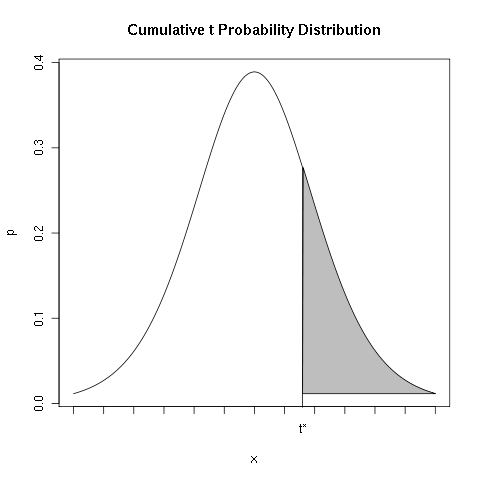
\includegraphics[width=6cm]{img/tcummulativeDist}
  
\end{frame}


\begin{frame}{\small $t$ distribution, cumulative distribution.}
  
  {
\fontencoding{T1}
\fontfamily{pcr}
\fontseries{m}
\fontshape{n}
\fontsize{5pt}{5pt}
\selectfont

\begin{tabular}{l|llllllllllll} 
t  & df= 5  &  6  &  7  &  8  &  9  &  10  &  11  &  12  &  13  &  14     \\\hline 
 0.0 & 0.5000 & 0.5000 & 0.5000 & 0.5000 & 0.5000 & 0.5000 & 0.5000 & 0.5000 & 0.5000 & 0.5000  \\[5pt] \arrayrulecolor{light-gray}\hline\arrayrulecolor{black}  
 0.1 & 0.4621 & 0.4618 & 0.4616 & 0.4614 & 0.4613 & 0.4612 & 0.4611 & 0.4610 & 0.4609 & 0.4609  \\[5pt] \arrayrulecolor{light-gray}\hline\arrayrulecolor{black}  
 0.2 & 0.4247 & 0.4240 & 0.4236 & 0.4232 & 0.4230 & 0.4227 & 0.4226 & 0.4224 & 0.4223 & 0.4222  \\[5pt] \arrayrulecolor{light-gray}\hline\arrayrulecolor{black}  
 0.3 & 0.3881 & 0.3871 & 0.3864 & 0.3859 & 0.3855 & 0.3852 & 0.3849 & 0.3847 & 0.3845 & 0.3843  \\[5pt] \arrayrulecolor{light-gray}\hline\arrayrulecolor{black}  
 0.4 & 0.3528 & 0.3515 & 0.3505 & 0.3498 & 0.3492 & 0.3488 & 0.3484 & 0.3481 & 0.3478 & 0.3476  \\[5pt] \arrayrulecolor{light-gray}\hline\arrayrulecolor{black}  
 0.5 & 0.3191 & 0.3174 & 0.3162 & 0.3153 & 0.3145 & 0.3139 & 0.3135 & 0.3131 & 0.3127 & 0.3124  \\[5pt] \arrayrulecolor{light-gray}\hline\arrayrulecolor{black}  
 0.6 & 0.2873 & 0.2852 & 0.2837 & 0.2826 & 0.2817 & 0.2809 & 0.2803 & 0.2798 & 0.2794 & 0.2790  \\[5pt] \arrayrulecolor{light-gray}\hline\arrayrulecolor{black}  
 0.7 & 0.2576 & 0.2551 & 0.2533 & 0.2519 & 0.2508 & 0.2499 & 0.2492 & 0.2486 & 0.2481 & 0.2477  \\[5pt] \arrayrulecolor{light-gray}\hline\arrayrulecolor{black}  
 0.8 & 0.2300 & 0.2271 & 0.2250 & 0.2234 & 0.2222 & 0.2212 & 0.2203 & 0.2196 & 0.2190 & 0.2185  \\[5pt] \arrayrulecolor{light-gray}\hline\arrayrulecolor{black}  
 0.9 & 0.2047 & 0.2014 & 0.1990 & 0.1972 & 0.1958 & 0.1946 & 0.1937 & 0.1929 & 0.1922 & 0.1917  \\[5pt] \arrayrulecolor{light-gray}\hline\arrayrulecolor{black}  
 1.0 & 0.1816 & 0.1780 & 0.1753 & 0.1733 & 0.1717 & 0.1704 & 0.1694 & 0.1685 & 0.1678 & 0.1671  \\[5pt] \arrayrulecolor{light-gray}\hline\arrayrulecolor{black}  
 1.1 & 0.1607 & 0.1567 & 0.1539 & 0.1517 & 0.1499 & 0.1486 & 0.1474 & 0.1465 & 0.1456 & 0.1449  \\[5pt] \arrayrulecolor{light-gray}\hline\arrayrulecolor{black}  
 1.2 & 0.1419 & 0.1377 & 0.1346 & 0.1322 & 0.1304 & 0.1289 & 0.1277 & 0.1266 & 0.1258 & 0.1250  \\[5pt] \arrayrulecolor{light-gray}\hline\arrayrulecolor{black}  
 1.3 & 0.1252 & 0.1207 & 0.1174 & 0.1149 & 0.1130 & 0.1114 & 0.1101 & 0.1090 & 0.1081 & 0.1073  \\[5pt] \arrayrulecolor{light-gray}\hline\arrayrulecolor{black}  
 1.4 & 0.1102 & 0.1055 & 0.1021 & 0.0995 & 0.0975 & 0.0959 & 0.0945 & 0.0934 & 0.0925 & 0.0916  \\[5pt] \arrayrulecolor{light-gray}\hline\arrayrulecolor{black}  
 1.5 & 0.0970 & 0.0921 & 0.0886 & 0.0860 & 0.0839 & 0.0823 & 0.0809 & 0.0797 & 0.0788 & 0.0779  \\[5pt] \arrayrulecolor{light-gray}\hline\arrayrulecolor{black}  
 1.6 & 0.0852 & 0.0804 & 0.0768 & 0.0741 & 0.0720 & 0.0703 & 0.0690 & 0.0678 & 0.0668 & 0.0660  \\[5pt] \arrayrulecolor{light-gray}\hline\arrayrulecolor{black}  
 1.7 & 0.0749 & 0.0700 & 0.0665 & 0.0638 & 0.0617 & 0.0600 & 0.0586 & 0.0574 & 0.0565 & 0.0556  \\[5pt] \arrayrulecolor{light-gray}\hline\arrayrulecolor{black}  
 1.8 & 0.0659 & 0.0610 & 0.0574 & 0.0548 & 0.0527 & 0.0510 & 0.0497 & 0.0485 & 0.0475 & 0.0467  \\[5pt] \arrayrulecolor{light-gray}\hline\arrayrulecolor{black}  
 1.9 & 0.0579 & 0.0531 & 0.0496 & 0.0470 & 0.0449 & 0.0433 & 0.0420 & 0.0409 & 0.0399 & 0.0391  \\[5pt] \arrayrulecolor{light-gray}\hline\arrayrulecolor{black}  
\end{tabular}

}

\end{frame}


\begin{frame}{\small $H_o:~\mu=3.0$, $H_a:~\mu>3.0$, $t^*=1.2$,
    $df=10$, find the $p$-value.}
{\small First, find the row for 1.2.}  
  {
\fontencoding{T1}
\fontfamily{pcr}
\fontseries{m}
\fontshape{n}
\fontsize{5pt}{5pt}
\selectfont

\begin{tabular}{l|llllllllllll} 
t  & df= 5  &  6  &  7  &  8  &  9  &  10  &  11  &  12  &  13  &  14     \\\hline 
 0.0 & 0.5000 & 0.5000 & 0.5000 & 0.5000 & 0.5000 & 0.5000 & 0.5000 & 0.5000 & 0.5000 & 0.5000  \\[5pt] \arrayrulecolor{light-gray}\hline\arrayrulecolor{black}  
 0.1 & 0.4621 & 0.4618 & 0.4616 & 0.4614 & 0.4613 & 0.4612 & 0.4611 & 0.4610 & 0.4609 & 0.4609  \\[5pt] \arrayrulecolor{light-gray}\hline\arrayrulecolor{black}  
 0.2 & 0.4247 & 0.4240 & 0.4236 & 0.4232 & 0.4230 & 0.4227 & 0.4226 & 0.4224 & 0.4223 & 0.4222  \\[5pt] \arrayrulecolor{light-gray}\hline\arrayrulecolor{black}  
 0.3 & 0.3881 & 0.3871 & 0.3864 & 0.3859 & 0.3855 & 0.3852 & 0.3849 & 0.3847 & 0.3845 & 0.3843  \\[5pt] \arrayrulecolor{light-gray}\hline\arrayrulecolor{black}  
 0.4 & 0.3528 & 0.3515 & 0.3505 & 0.3498 & 0.3492 & 0.3488 & 0.3484 & 0.3481 & 0.3478 & 0.3476  \\[5pt] \arrayrulecolor{light-gray}\hline\arrayrulecolor{black}  
 0.5 & 0.3191 & 0.3174 & 0.3162 & 0.3153 & 0.3145 & 0.3139 & 0.3135 & 0.3131 & 0.3127 & 0.3124  \\[5pt] \arrayrulecolor{light-gray}\hline\arrayrulecolor{black}  
 0.6 & 0.2873 & 0.2852 & 0.2837 & 0.2826 & 0.2817 & 0.2809 & 0.2803 & 0.2798 & 0.2794 & 0.2790  \\[5pt] \arrayrulecolor{light-gray}\hline\arrayrulecolor{black}  
 0.7 & 0.2576 & 0.2551 & 0.2533 & 0.2519 & 0.2508 & 0.2499 & 0.2492 & 0.2486 & 0.2481 & 0.2477  \\[5pt] \arrayrulecolor{light-gray}\hline\arrayrulecolor{black}  
 0.8 & 0.2300 & 0.2271 & 0.2250 & 0.2234 & 0.2222 & 0.2212 & 0.2203 & 0.2196 & 0.2190 & 0.2185  \\[5pt] \arrayrulecolor{light-gray}\hline\arrayrulecolor{black}  
 0.9 & 0.2047 & 0.2014 & 0.1990 & 0.1972 & 0.1958 & 0.1946 & 0.1937 & 0.1929 & 0.1922 & 0.1917  \\[5pt] \arrayrulecolor{light-gray}\hline\arrayrulecolor{black}  
 1.0 & 0.1816 & 0.1780 & 0.1753 & 0.1733 & 0.1717 & 0.1704 & 0.1694 & 0.1685 & 0.1678 & 0.1671  \\[5pt] \arrayrulecolor{light-gray}\hline\arrayrulecolor{black}  
 1.1 & 0.1607 & 0.1567 & 0.1539 & 0.1517 & 0.1499 & 0.1486 & 0.1474 & 0.1465 & 0.1456 & 0.1449  \\[5pt] \arrayrulecolor{light-gray}\hline\arrayrulecolor{black}  
\rowcolor{light-red} 1.2 & 0.1419 & 0.1377 & 0.1346 & 0.1322 & 0.1304 & 0.1289 & 0.1277 & 0.1266 & 0.1258 & 0.1250  \\[5pt] \arrayrulecolor{light-gray}\hline\arrayrulecolor{black}  
 1.3 & 0.1252 & 0.1207 & 0.1174 & 0.1149 & 0.1130 & 0.1114 & 0.1101 & 0.1090 & 0.1081 & 0.1073  \\[5pt] \arrayrulecolor{light-gray}\hline\arrayrulecolor{black}  
 1.4 & 0.1102 & 0.1055 & 0.1021 & 0.0995 & 0.0975 & 0.0959 & 0.0945 & 0.0934 & 0.0925 & 0.0916  \\[5pt] \arrayrulecolor{light-gray}\hline\arrayrulecolor{black}  
 1.5 & 0.0970 & 0.0921 & 0.0886 & 0.0860 & 0.0839 & 0.0823 & 0.0809 & 0.0797 & 0.0788 & 0.0779  \\[5pt] \arrayrulecolor{light-gray}\hline\arrayrulecolor{black}  
 1.6 & 0.0852 & 0.0804 & 0.0768 & 0.0741 & 0.0720 & 0.0703 & 0.0690 & 0.0678 & 0.0668 & 0.0660  \\[5pt] \arrayrulecolor{light-gray}\hline\arrayrulecolor{black}  
 1.7 & 0.0749 & 0.0700 & 0.0665 & 0.0638 & 0.0617 & 0.0600 & 0.0586 & 0.0574 & 0.0565 & 0.0556  \\[5pt] \arrayrulecolor{light-gray}\hline\arrayrulecolor{black}  
 1.8 & 0.0659 & 0.0610 & 0.0574 & 0.0548 & 0.0527 & 0.0510 & 0.0497 & 0.0485 & 0.0475 & 0.0467  \\[5pt] \arrayrulecolor{light-gray}\hline\arrayrulecolor{black}  
 1.9 & 0.0579 & 0.0531 & 0.0496 & 0.0470 & 0.0449 & 0.0433 & 0.0420 & 0.0409 & 0.0399 & 0.0391  \\[5pt] \arrayrulecolor{light-gray}\hline\arrayrulecolor{black}  
\end{tabular}

}

\end{frame}


\begin{frame}{\small $H_o:~\mu=3.0$, $H_a:~\mu>3.0$, $t^*=1.2$,
    $df=10$, find the $p$-value.}
{\small First, find the row for 1.2. Next find the column for $df=10$.}    
  {
\fontencoding{T1}
\fontfamily{pcr}
\fontseries{m}
\fontshape{n}
\fontsize{5pt}{5pt}
\selectfont

\begin{tabular}{l|lllll>{\columncolor{light-blue}}lllllll} 
t  & df= 5  &  6  &  7  &  8  &  9  &  10  &  11  &  12  &  13  &  14    \\\hline 
 0.0 & 0.5000 & 0.5000 & 0.5000 & 0.5000 & 0.5000 & 0.5000 & 0.5000 & 0.5000 & 0.5000 & 0.5000  \\[5pt] \arrayrulecolor{light-gray}\hline\arrayrulecolor{black}  
 0.1 & 0.4621 & 0.4618 & 0.4616 & 0.4614 & 0.4613 & 0.4612 & 0.4611 & 0.4610 & 0.4609 & 0.4609  \\[5pt] \arrayrulecolor{light-gray}\hline\arrayrulecolor{black}  
 0.2 & 0.4247 & 0.4240 & 0.4236 & 0.4232 & 0.4230 & 0.4227 & 0.4226 & 0.4224 & 0.4223 & 0.4222  \\[5pt] \arrayrulecolor{light-gray}\hline\arrayrulecolor{black}  
 0.3 & 0.3881 & 0.3871 & 0.3864 & 0.3859 & 0.3855 & 0.3852 & 0.3849 & 0.3847 & 0.3845 & 0.3843  \\[5pt] \arrayrulecolor{light-gray}\hline\arrayrulecolor{black}  
 0.4 & 0.3528 & 0.3515 & 0.3505 & 0.3498 & 0.3492 & 0.3488 & 0.3484 & 0.3481 & 0.3478 & 0.3476  \\[5pt] \arrayrulecolor{light-gray}\hline\arrayrulecolor{black}  
 0.5 & 0.3191 & 0.3174 & 0.3162 & 0.3153 & 0.3145 & 0.3139 & 0.3135 & 0.3131 & 0.3127 & 0.3124  \\[5pt] \arrayrulecolor{light-gray}\hline\arrayrulecolor{black}  
 0.6 & 0.2873 & 0.2852 & 0.2837 & 0.2826 & 0.2817 & 0.2809 & 0.2803 & 0.2798 & 0.2794 & 0.2790  \\[5pt] \arrayrulecolor{light-gray}\hline\arrayrulecolor{black}  
 0.7 & 0.2576 & 0.2551 & 0.2533 & 0.2519 & 0.2508 & 0.2499 & 0.2492 & 0.2486 & 0.2481 & 0.2477  \\[5pt] \arrayrulecolor{light-gray}\hline\arrayrulecolor{black}  
 0.8 & 0.2300 & 0.2271 & 0.2250 & 0.2234 & 0.2222 & 0.2212 & 0.2203 & 0.2196 & 0.2190 & 0.2185  \\[5pt] \arrayrulecolor{light-gray}\hline\arrayrulecolor{black}  
 0.9 & 0.2047 & 0.2014 & 0.1990 & 0.1972 & 0.1958 & 0.1946 & 0.1937 & 0.1929 & 0.1922 & 0.1917  \\[5pt] \arrayrulecolor{light-gray}\hline\arrayrulecolor{black}  
 1.0 & 0.1816 & 0.1780 & 0.1753 & 0.1733 & 0.1717 & 0.1704 & 0.1694 & 0.1685 & 0.1678 & 0.1671  \\[5pt] \arrayrulecolor{light-gray}\hline\arrayrulecolor{black}  
 1.1 & 0.1607 & 0.1567 & 0.1539 & 0.1517 & 0.1499 & 0.1486 & 0.1474 & 0.1465 & 0.1456 & 0.1449  \\[5pt] \arrayrulecolor{light-gray}\hline\arrayrulecolor{black}  
\rowcolor{light-red} 1.2 & 0.1419 & 0.1377 & 0.1346 & 0.1322 & 0.1304 & 0.1289 & 0.1277 & 0.1266 & 0.1258 & 0.1250  \\[5pt] \arrayrulecolor{light-gray}\hline\arrayrulecolor{black}  
 1.3 & 0.1252 & 0.1207 & 0.1174 & 0.1149 & 0.1130 & 0.1114 & 0.1101 & 0.1090 & 0.1081 & 0.1073  \\[5pt] \arrayrulecolor{light-gray}\hline\arrayrulecolor{black}  
 1.4 & 0.1102 & 0.1055 & 0.1021 & 0.0995 & 0.0975 & 0.0959 & 0.0945 & 0.0934 & 0.0925 & 0.0916  \\[5pt] \arrayrulecolor{light-gray}\hline\arrayrulecolor{black}  
 1.5 & 0.0970 & 0.0921 & 0.0886 & 0.0860 & 0.0839 & 0.0823 & 0.0809 & 0.0797 & 0.0788 & 0.0779  \\[5pt] \arrayrulecolor{light-gray}\hline\arrayrulecolor{black}  
 1.6 & 0.0852 & 0.0804 & 0.0768 & 0.0741 & 0.0720 & 0.0703 & 0.0690 & 0.0678 & 0.0668 & 0.0660  \\[5pt] \arrayrulecolor{light-gray}\hline\arrayrulecolor{black}  
 1.7 & 0.0749 & 0.0700 & 0.0665 & 0.0638 & 0.0617 & 0.0600 & 0.0586 & 0.0574 & 0.0565 & 0.0556  \\[5pt] \arrayrulecolor{light-gray}\hline\arrayrulecolor{black}  
 1.8 & 0.0659 & 0.0610 & 0.0574 & 0.0548 & 0.0527 & 0.0510 & 0.0497 & 0.0485 & 0.0475 & 0.0467  \\[5pt] \arrayrulecolor{light-gray}\hline\arrayrulecolor{black}  
 1.9 & 0.0579 & 0.0531 & 0.0496 & 0.0470 & 0.0449 & 0.0433 & 0.0420 & 0.0409 & 0.0399 & 0.0391  \\[5pt] \arrayrulecolor{light-gray}\hline\arrayrulecolor{black}  
\end{tabular}

}

\end{frame}



% LocalWords:  Clarkson pausesection hideallsubsections
